\documentclass[12pt,a4paper,openany]{scrbook}

\include{Allgemein/packages}
\include{Allgemein/commands}

\addbibresource{bib/literature.bib}



%------------------------------------Links-----------------------------------------------------------------------%
\newcommand{\linkPi}{https://www.reichelt.de/raspberry-pi-3-b-4x-1-4-ghz-1-gb-ram-wlan-bt-raspberry-pi-3b--p217696.html}

\newcommand{\linkPiNT}{https://www.reichelt.de/raspberry-pi-netzteil-5-v-2-5-a-micro-usb-schwarz-nt-musb-25-sw-p167078.html}

\newcommand{\linkMstick}{https://eckstein-shop.de/M5StackM5StickCPLUSESP32-PICOMiniIoTDevelopmentKit2CInfrared2FRTC2FMic2FLED2FIMU2FPMU}

\newcommand{\linkBuzzer}{https://www.reichelt.de/sg/de/entwicklerboards-aktives-piezo-buzzer-modul-debo-piezo-p239111.html}


\begin{document}
	
	\include{Kapitel/titlepage} 
	\newpage
\chapter*{Hardwarebeschreibung Raspberry Pi}

\section{Einleitung: Vorstellung Raspberry Pi}
Der Raspberry Pi ist ein opensource Minicomputer, welcher ursprünglich als kostengünstiges System für Lernzwecke im Bereich der Programmierung gedacht war. [1]  \\
Besonders in der Makerszene erfreut sich der Raspberry Pi einer großen Beliebtheit. Es sind Projekte vom Desktopcomputer [1] bis hin zur Steuerung und Überwachung heimischer 3D-Drucker [2] realisierbar.\\ 
%Das Produktprotfolio reicht vom leistungsschwächeren Raspberry Pi (1Ghz singlecore, 512 MB RAM) zum leistungsstärkeren Raspberry Pi 
\\[3mm]


	\begin{figure}[!h]
	\centering
	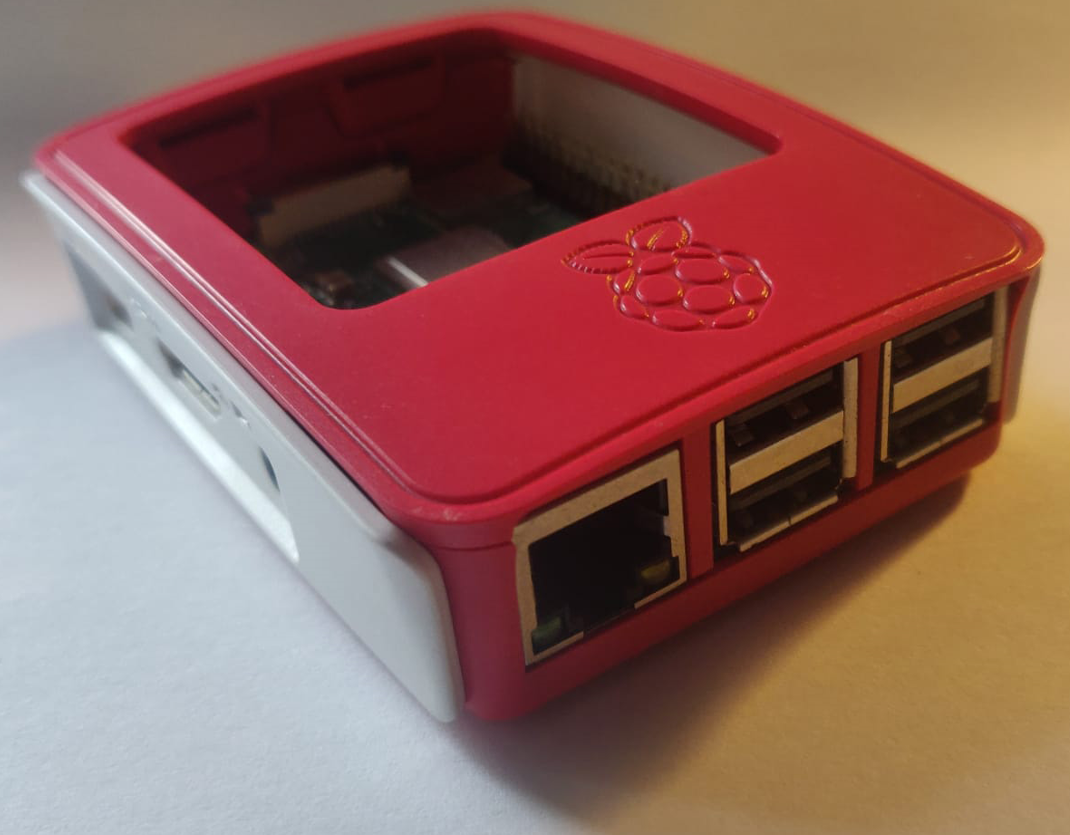
\includegraphics[height=250pt]{img/pi_mitgehaeuse.png}
	\caption{Bildtitel}
	\label{Bildlabel}
\end{figure}	


\chapter{Raspberry Pi für das Projekt}
Für das Projekt Überwachungssystem mittels der IMU des M5 Sticks soll ein\\ 
Raspberry Pi 3B+ als sogenannter IoT Broker und als Aktor für den Alarm genutzt werden.\\
%Das Modell 3B+ verfügt über eine Rechenleistung von
Der Raspberry Pi 3B+ wurde für das Projekt am Geeignetsten eingestuft, da er im Gegensatz zu seinen Vorgängermodellen ... und der preisliche Unterschied relativ zur gebotenen Leistung sehr marginal ist.  

	\begin{figure}[!h]
	\centering
	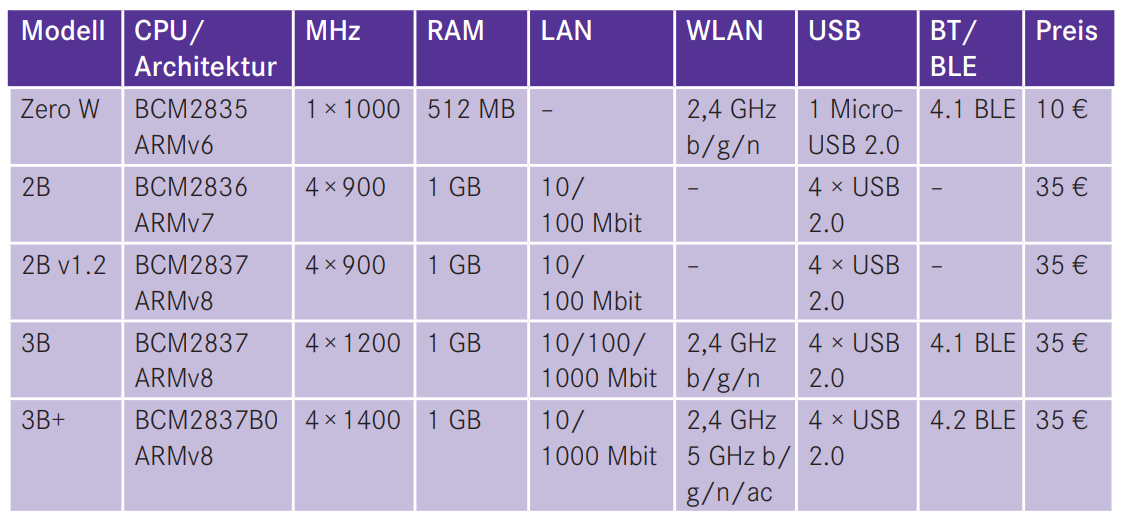
\includegraphics[height=200pt]{img/tabelle_pi_vergleich}
	\caption{Bildtitel}
	\label{Bildlabel}
\end{figure}


\section{Anschlussmöglichkeiten Anhand Raspberry Pi 3B+}
Der Raspberry Pi 3B+ verfügt im Allgemeinen über folgende Anschlussmöglichkeiten:\\[3mm] 
$\bullet$ HDMI   \\ %\hspace{20pt} $\bullet$ 
$\bullet$ 3,5mm AUX\\ 
$\bullet$ 4 $\times$ USB 2.0 \\ 
$\bullet$ Ethernet 1Gbit/RJ45\\ 
$\bullet$ CCI (Camera Connector Interface)\\ 
$\bullet$  DSI (Display Serial Interface)\\
$\bullet$ 40 GPIO-Pins\\
$\bullet$ Steckplatz für die microSD-Karte\\
$\bullet$ Micro-USB Anschluss für die Stromversorgung des PIs\\
Quelle: IOT at Home S.60\\ [10mm]

	\begin{figure}[!h]
		\centering
		\includegraphics[height=250pt]{img/raspberry_pi3b.pdf}
		\caption{Bildtitel}
		\label{Bildlabel}
	\end{figure}
Für das Projekt sind insbesondere die GPIO-Pins und der Ethernetport von Bedeutung.\\ 
  

\section{Weitere Hardware, die für den Betrieb des Pis benötigt wird}
\subsection{Piezo Buzzer}

\subsection{Netzteil}
\vspace{1cm}
\centering

\chapter{Quellen}
[1]https://www.raspberrypi.org/help/what-%20is-a-raspberry-pi/ 

[2]001\\ 

[3]https://octoprint.org/

\end{document}
